\documentclass[spanish,xcolor=dvipsnames]{beamer}
    \usefonttheme{professionalfonts}
    \usetheme{Copenhagen}
    \usecolortheme[named=NavyBlue]{structure}
    \setbeamersize{text margin left=1em,text margin right=1.5em}
    \setbeamercovered{transparent}
    \setbeamertemplate{sections/subsections in toc}[circle]
    %\setbeamertemplate{itemize items}[bullet]
    %\setbeamertemplate{itemize subitem}[square]
    %\setbeamertemplate{enumerate items}[square]
    \setbeamertemplate{navigation symbols}{}
    \setbeamertemplate{headline}{}
	
    \usepackage[spanish]{babel}
    \usepackage[T1]{fontenc}
    \usepackage[utf8]{inputenc}
    
	%Estos paquetes pueden ser útiles,
	%si no están instalados puede quitarlos,
%%	%si los necesita instálelos
    \usepackage{ragged2e}
    \usepackage{lmodern}
    \usepackage[font=scriptsize,labelfont=bf,center]{caption}
    \usepackage{float}
    \usepackage{graphicx}
    \usepackage{subfig}
    \usepackage{multicol}
    \usepackage{amsmath}
    \usepackage{tikz}
    \usetikzlibrary{%
                    automata,%
                    arrows,%
                    shapes,%
                    chains,%
                    matrix,%
                    plotmarks,%
                    %pgfplots.units,%
                    decorations.markings,%
                    decorations.pathmorphing,%
                    backgrounds,%
                    scopes,%
                    calc,%
                    petri,%
                    positioning,%
                    fit%
                    }%
    \usepgflibrary{arrows}
    \usepackage{pgfplots}
    \renewcommand{\shorthandsspanish}{}
    \renewcommand{\spanishtablename}{Tabla}
%    \spanishdecimal{,}

    \makeatletter
        \defbeamertemplate*{footline}{jtheme}
        {
          \leavevmode%
          \hbox{%
          \begin{beamercolorbox}[wd=.25\paperwidth,ht=2.25ex,dp=1ex,center]{author in head/foot}%
            \usebeamerfont{author in head/foot}\insertshortauthor~~\beamer@ifempty{\insertshortinstitute}{}
            {(\insertshortinstitute)}
          \end{beamercolorbox}%
          \begin{beamercolorbox}[wd=.50\paperwidth,ht=2.25ex,dp=1ex,center]{title in head/foot}%
            \usebeamerfont{title in head/foot}\insertshorttitle
          \end{beamercolorbox}%
          \begin{beamercolorbox}[wd=.25\paperwidth,ht=2.25ex,dp=1ex,right]{date in head/foot}%
            \usebeamerfont{date in head/foot}\insertshortdate{}\hspace*{2em}
            \insertframenumber{} / \inserttotalframenumber\hspace*{2ex}
          \end{beamercolorbox}}%
          \vskip0pt%
        }
    \makeatother

\DeclareMathOperator*{\argmin}{arg\ min}
\DeclareMathOperator*{\argmax}{arg\ max}

    %%-------------------Portada-------------------------%%
    \title[Sistema Web GALATEA]{\sc Diseño e implementación de un Sistema Web para el Simulador de Eventos Discretos GALATEA}
    \author[Erik Velásquez ]{ Erik Velasquez}
    \institute[ULA]{
        Facultad de Ingeniería\\Escuela de Ingeniería de Sistemas\\Trabajo de Grado
    }
    \date[Diciembre 2016]{\footnotesize Mérida, 09 de diciembre, 2016}

    %%-------------------Fin-Portada---------------------%%

\begin{document}
	%%--------------------Diapositiva--------------------%%
    \begin{frame}[plain] % [plain] para que no salga el contenido en esta página
	    \begin{center}
	    	
\includegraphics[width=1.5cm]{ULA_logo_titulo}
	    \end{center}
	    \titlepage
    \end{frame}
    %%------------------------Fin------------------------%%
	
	%Logo de la esquina superior derecha de cada frame, necesita tres compilaciones para actualizar.
	\addtobeamertemplate{frametitle}{}{%
    \begin{tikzpicture}[remember picture,overlay]
    	\node[anchor=north east,yshift=11pt,xshift=11pt] at (current page.north east) {
\includegraphics[height=1.5cm,angle=-20,keepaspectratio]{ula}};
    \end{tikzpicture}}
    
	%%--------------------Diapositiva--------------------%%
    \begin{frame}\justifying
        \frametitle{Agenda}
        \begin{columns}
            \begin{column}{0.0cm}
            \end{column}
            \begin{column}{0.9\textwidth}
                \tableofcontents
            \end{column}
        \end{columns}
    \end{frame}
    %%------------------------Fin------------------------%%
    
    %%--------------------Diapositiva--------------------%%
    \section{Introducción}
    \begin{frame}
    	\frametitle{Introducción}
    	\framesubtitle{Planteamiento del Problema}
    	
    	\begin{itemize}
    		\item No se dispone de una plataforma web acondicionada para que, de manera fácil y rápida se pueda hacer uso del simulador GALATEA.
    		\item Los usuarios y usuarias del Centro de Simulación y Modelado (CESIMO) de la Universidad de los Andes, suelen tener muchas dificultades para ejecutar los modelos de simulación en el simulador GALATEA.
    	\end{itemize}

    \end{frame}
    \begin{frame}
    	\frametitle{Introducción}
    	\framesubtitle{Justificación}
    	
    	\begin{itemize}
    		\item Desarrollar un sistema web que sirva como base para la simulación de eventos discretos.
    		\item Sistema web amplíe la base de usuarios y usuarias del simulador.
    		\item Ponerlos en contacto con diferentes expertos que trabajan en el CESIMO.
    		\item Hacer que el simulador sea amigable a la web, para así, aprovechar todas las ventajas que nos proporciona.
    	\end{itemize}
    	
    \end{frame}
    \begin{frame}
    	\frametitle{Introducción}
    	\framesubtitle{Objetivo General}
    	
    	Diseñar e implementar un sistema web para los usuarios y usuarias, modelistas y simulistas  del simulador de eventos discretos GALATEA, que les permita realizar todas las tareas habituales de modelado, codificación y análisis en sus computadores y en la forma que prefieran, pero permitiéndoles realizar las tareas automáticas de compilación, gestión de archivos, simulación y gestión de salidas, en el espacio virtual y con los recursos compartidos de un servidor Web.
    	
    \end{frame}
    \begin{frame}
    	\frametitle{Introducción}
    	\framesubtitle{Objetivos Específicos}
    	
    	\begin{itemize}
    		\item Desarrollar un sistema web que permita el control de usuarios junto con los roles a ser utilizados en el sistema.
    		\item Diseñar e implementar una arquitectura de software que permita la comunicación entre el software de simulación y el sistema web.
    		\item Instalar y configurar en un servidor la arquitectura de software para el sistema de simulación.
    		\item Incorporar el simulador GALATEA como servicio para el sistema web.
    		\item Diseñar y desarrollar un cliente GUI/controlador para un modelo que se pueda gestionar archivos y simular con GALATEA a través del sistema web desarrollado.
    		\item Sistematizar la experiencia de uso del sistema web para simulación.
    		\item Analizar el sistema web desarrollado y establecer las conclusiones.
    	\end{itemize}
    	
    \end{frame}
    \begin{frame}
    	\frametitle{Introducción}
    	\framesubtitle{Resumen}
    	
    	\begin{itemize}
    		\item GALATEA.
    		\item Control de Usuarios.
    		\item Desarrollo de un Sistema Web.
    		\item Integración del Sistema Web y GALATEA.
    	\end{itemize}
    	
    \end{frame}
    %%------------------------Fin------------------------%%
    
    %%--------------------Diapositiva--------------------%%
    \section{Desarrollo del Sistema Web}
    \begin{frame}
    	\frametitle{Desarrollo del Sistema Web}
    	%%\framesubtitle{Subtítulo del frame (no obligatorio)}
    	
    	\begin{columns}
    		\begin{column}{.5\linewidth}
    			\begin{itemize}
    				\item La aplicación Web que funciona como coordinador del sistema, control de usuarios y roles.
    				\item Administración de archivos.
    				\item El Sistema de Integración con GALATEA.
    			\end{itemize}
    		\end{column}
    		\begin{column}{.5\linewidth}
    			\begin{figure}[H]
    				\centering
    				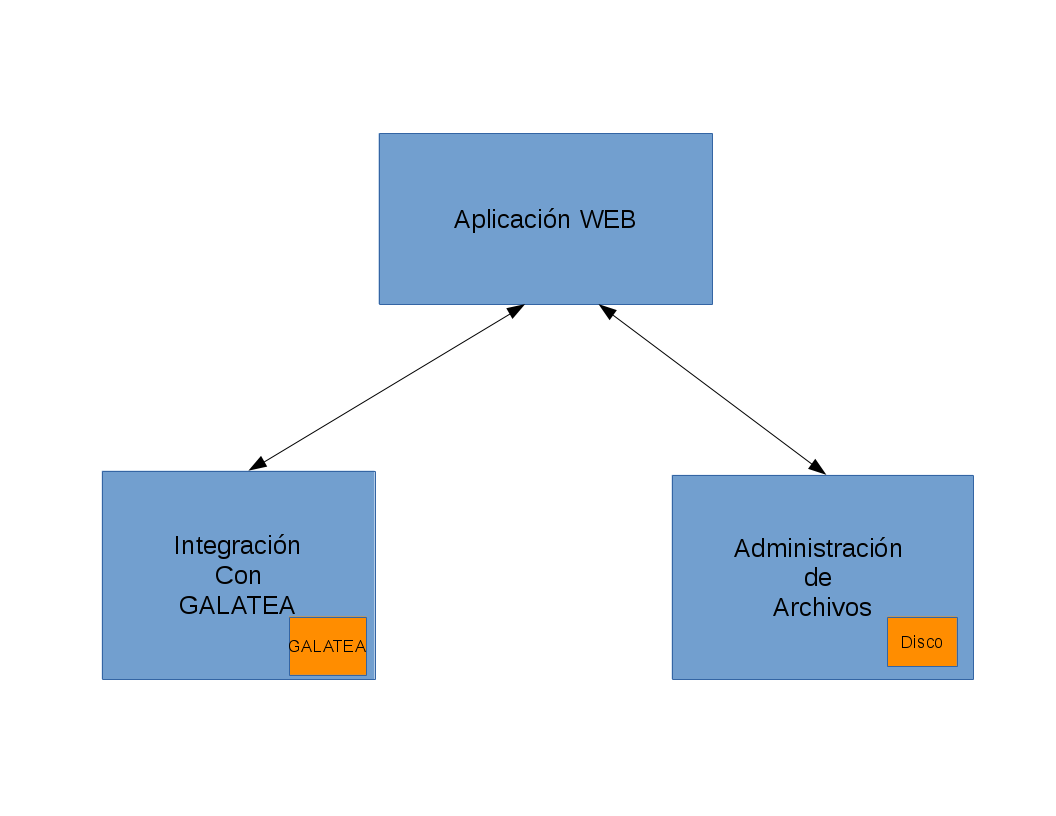
\includegraphics[scale=0.23]{img/estructuraSistema.png}
    				\caption{Sistema de Simulación Web GALATEA.}
    				\label{estructuraSistema}
    			\end{figure}
    		\end{column}
    	\end{columns}
    	
    \end{frame}
    \begin{frame}
    	\frametitle{Desarrollo del Sistema Web}
    	\framesubtitle{Diseño de la Aplicación}
    	
    	\begin{columns}
    		\begin{column}{.7\linewidth}
    			\begin{figure}[H]
    				\centering
    				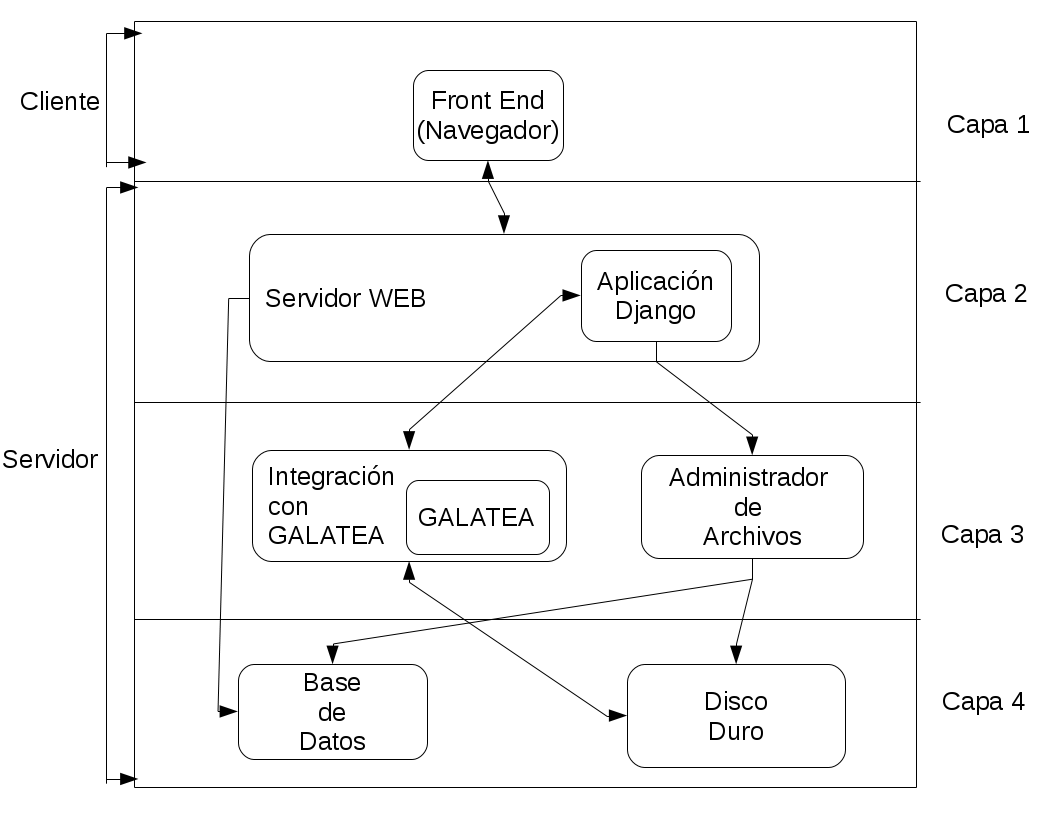
\includegraphics[scale=0.29]{img/arquitecturaAplicacion.png}
    				\caption{Arquitectura de la aplicación web.}
    				\label{arquitecturaAplicacion}
    			\end{figure}
    		\end{column}
    		\begin{column}{.3\linewidth}
    			\begin{itemize}
    				\item Presentación.
    				\item Servidor Web.
    				\item Integración de Procesos.
    				\item Datos.
    			\end{itemize}
    		\end{column}
    		
    	\end{columns}
    	
    \end{frame}
    \begin{frame}
    	\frametitle{Desarrollo del Sistema Web}
    	\framesubtitle{Características de la Aplicación}
    	
    	\begin{itemize}
    		\item Diseño modular.
    		\item Validación y verificación de cada módulo.
    		\item Arquitectura por capas.
    	\end{itemize}
    	
    \end{frame}
    \begin{frame}
    	\frametitle{Desarrollo del Sistema Web}
    	\framesubtitle{Diseño de la base de datos}
    	
    	\begin{itemize}
    		\item Control de usuarios: Registro, ingresos, perfiles y relaciones.
    		\item Control de archivos y carpetas: Creación, actualización, ubicación, espacio ocupado.
    	\end{itemize}
    	
    \end{frame}
    \begin{frame}
    	\frametitle{Desarrollo del Sistema Web}
    	\framesubtitle{Diseño de la base de datos (USUARIOS)}
    	
    	\begin{figure}[H]
    		\centering
    		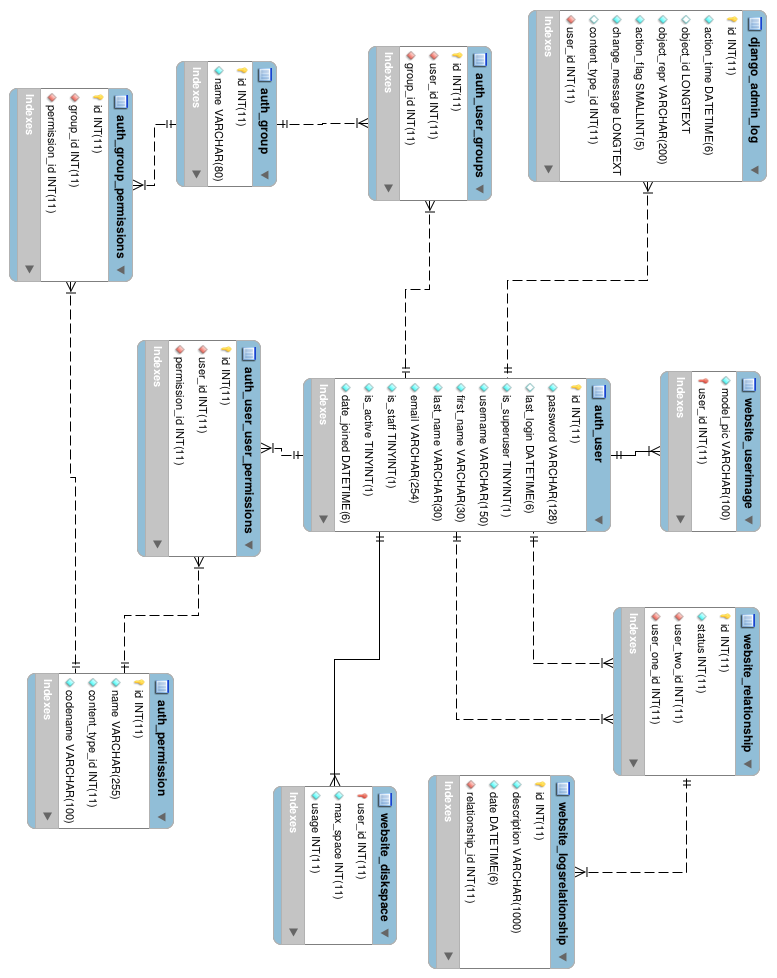
\includegraphics[scale=0.25]{img/usuariosDB.png}
    		\caption{Entidades manejo de usuarios.}
    		\label{entidadRelacionUsuarios}
    	\end{figure}
    	
    \end{frame}
    \begin{frame}
    	\frametitle{Desarrollo del Sistema Web}
    	\framesubtitle{Diseño de la base de datos (ARCHIVOS)}
    	
    	\begin{figure}[H]
    		\centering
    		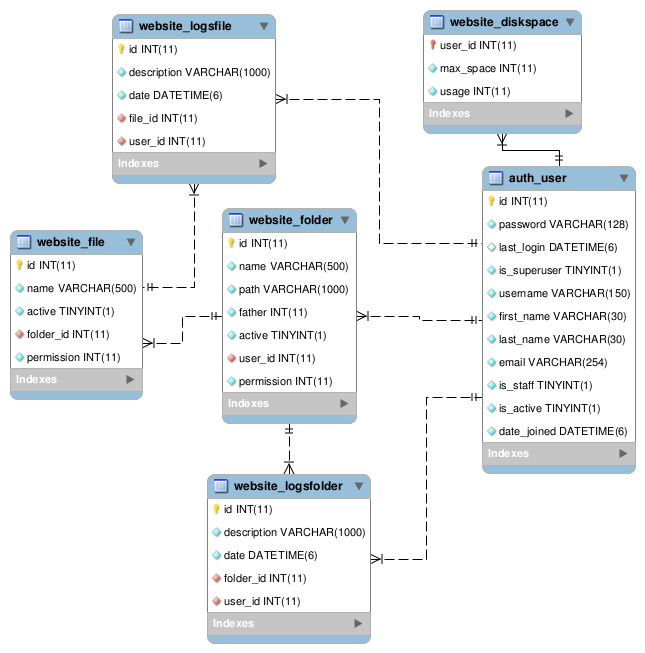
\includegraphics[scale=0.3]{img/archivosDB.png}
    		\caption{Entidades manejo archivos y carpetas.}
    		\label{entidadRelacionArchivosCarpetas}
    	\end{figure}
    	
    \end{frame}
    \begin{frame}
    	\frametitle{Desarrollo del Sistema Web}
    	\framesubtitle{Diseño de Pantallas}
    	
    	\begin{itemize}
    		\item Micro-lenguaje de plantillas.
    		\item Paradigma del diseño web adaptable.
    		\item Estructura de plantilla:
    		\begin{itemize}
    			\item (1) Bloque de título.
    			\item (2) Bloque de navegación.
    			\item (3) Bloque de contenido.
    			\item (4) Bloque de JavaScript.
    		\end{itemize}
    	\end{itemize}
    	
    \end{frame}
    \begin{frame}
    	\frametitle{Desarrollo del Sistema Web}
    	\framesubtitle{Diseño de Pantallas}
    	
    	\begin{figure}[H]
    		\centering
    		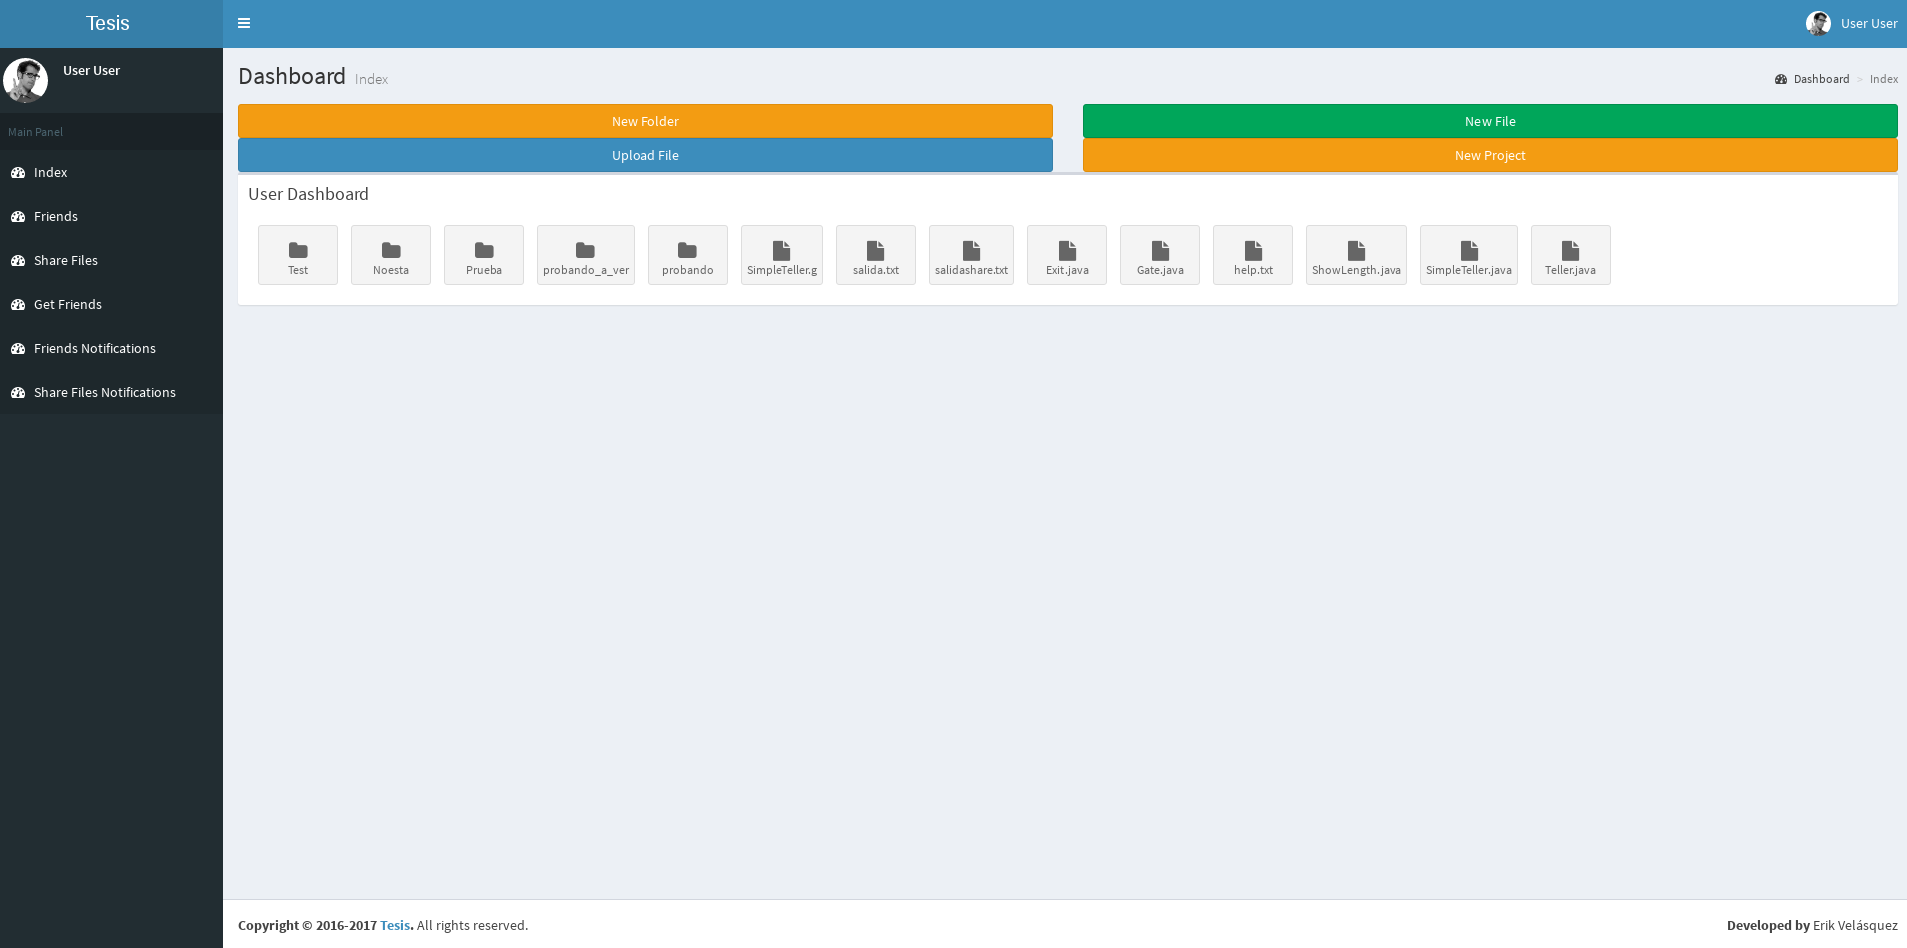
\includegraphics[scale=0.17]{img/pantallaInicio.png}
    		\caption{Pantalla del Dashboard (Inicio).}
    		\label{pantalla1}
    	\end{figure}
    	
    \end{frame}
    \begin{frame}
    	\frametitle{Desarrollo del Administrador de Archivos}
    	\framesubtitle{Diseño y Estructura}
    	
    	\begin{figure}[H]
    		\centering
    		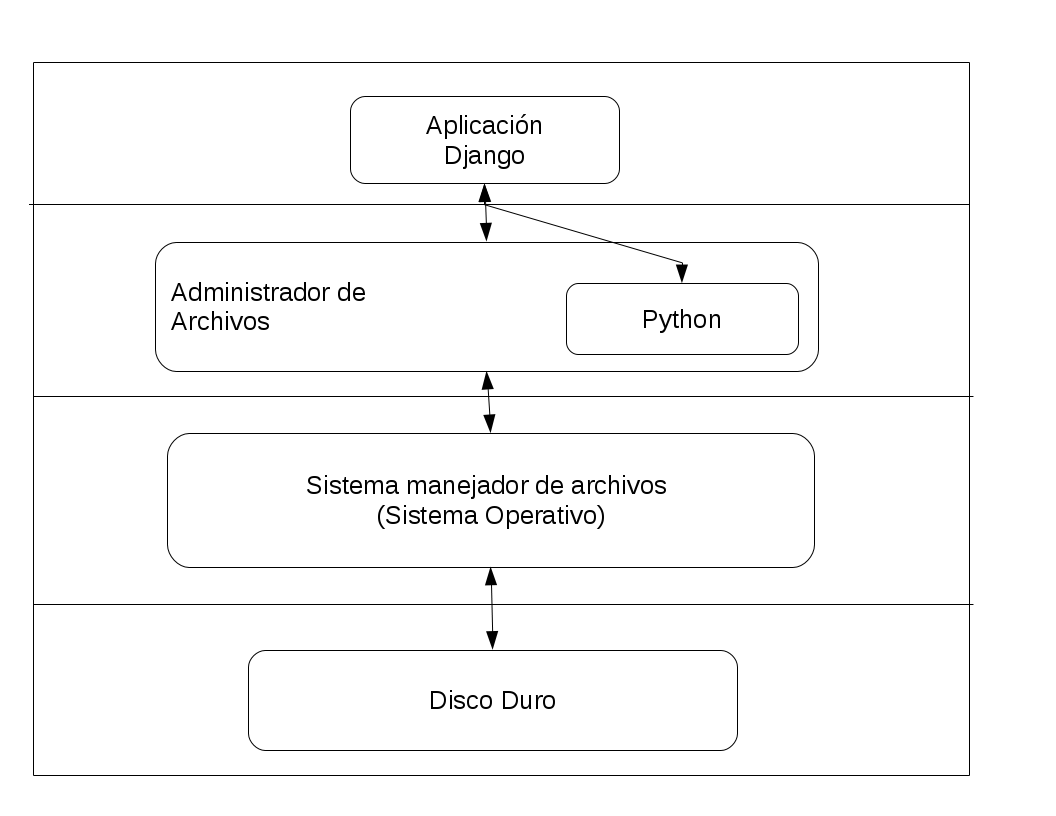
\includegraphics[scale=0.27]{img/estructuraArchivosCarpetas.png}
    		\caption{Estructura del Administrador de Archivos y Carpetas.}
    		\label{estructuraAdministradorArchivosCarpetas}
    	\end{figure}
    	
    \end{frame}
    \begin{frame}
    	\frametitle{Desarrollo del Administrador de Archivos}
    	\framesubtitle{Control de Archivos y Carpetas}
    	
    	\begin{columns}
    		\begin{column}{.3\linewidth}
    			\begin{itemize}
    				\item Archivos.
    				\begin{itemize}
    					\item Create File.
    					\item Show File.
    					\item Edit File.
    					\item Move File.
    					\item Delete File.
    				\end{itemize}
    				\item Carpetas.
    				\begin{itemize}
    					\item Create Folder.
    					\item Show Folder.
    					\item Edit Folder.
    					\item Move Folder.
    					\item Delete Folder.
    				\end{itemize}
    			\end{itemize}
    		\end{column}
    		\begin{column}{.7\linewidth}
    			\begin{figure}[H]
    				\centering
    				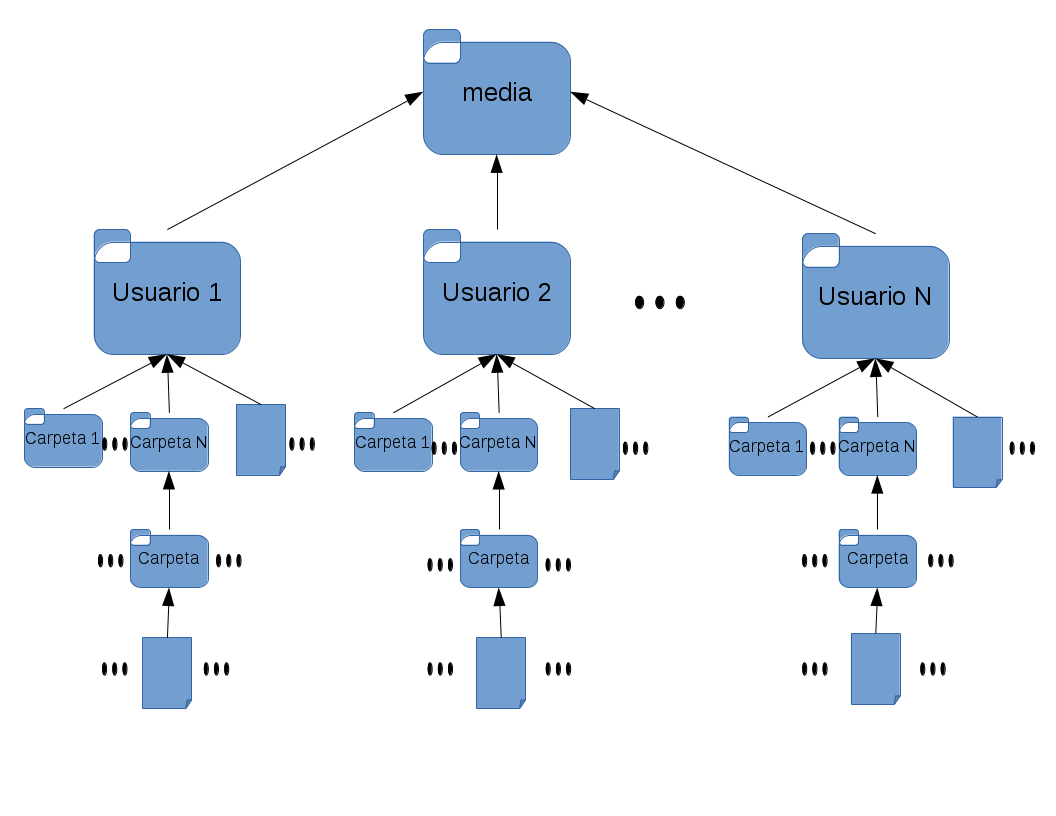
\includegraphics[scale=0.25]{img/jerarquiaCarpetas.png}
    				\caption{Jerarquía de Carpetas.}
    				\label{jerarquiaCarpetas}
    			\end{figure}
    		\end{column}
    	\end{columns}
    \end{frame}
    \begin{frame}
    	\frametitle{Desarrollo del Administrador de Archivos}
    	\framesubtitle{Características del Control de Archivos y Carpetas}
    	
    	\begin{itemize}
    		\item Espacio en disco físico es limitado.
    		\item Cada usuario tiene una porción de espacio asociado.
    		\item Espacio es constantemente monitoreado.
    		\item Se desarrolló usando llamadas a Sistema Operativo.
    		\item Uso de las nuevas tecnologías disponibles como: "hot swap", entre otros.
    	\end{itemize}
    \end{frame}
    \begin{frame}
    	\frametitle{Desarrollo del Administrador de Archivos}
    	\framesubtitle{Control de Permisos}
    	
    	\begin{itemize}
    		\item Usuarios Amigos.
    		\item Usuarios NO Amigos.
    		\item Permisología.
    		\begin{itemize}
    			\item Private.
    			\item Show.
    			\item Edit.
    			\item Public.
    		\end{itemize}
    	\end{itemize}
    \end{frame}
    \begin{frame}
    	\frametitle{Desarrollo del Sistema Web}
    	\framesubtitle{Resumen}
    	
    	\begin{itemize}
    		\item Arquitectura.
    		\item Herramientas de Desarrollo.
    		\item Control de Usuarios.
    		\item Control de Archivos.
    	\end{itemize}
    	
    \end{frame}
    
    %%------------------------Fin------------------------%%
    
    %%--------------------Diapositiva--------------------%%
    \section{Integración de GALATEA}
    \begin{frame}
    	\frametitle{Integración de GALATEA}
    	%%\framesubtitle{Subtítulo del frame (no obligatorio)}
    	
    	\begin{itemize}
    		\item Subprocesos:
    		\begin{itemize}
    			\item Invocación a un subproceso o proceso externo, enviándole los parámetros necesarios para su ejecución.
    		\end{itemize}
    		\item Sockets:
    		\begin{itemize}
    			\item Peticiones en un puerto de comunicación específico, lo cual nos permite comunicar nuestro sistema Python con el motor de simulación escrito en Java.
    		\end{itemize}
    	\end{itemize}
    \end{frame}
    \begin{frame}
    	\frametitle{Integración de GALATEA}
    	\framesubtitle{Integración Subprocesos}
    	
    	\begin{figure}[H]
    		\centering
    		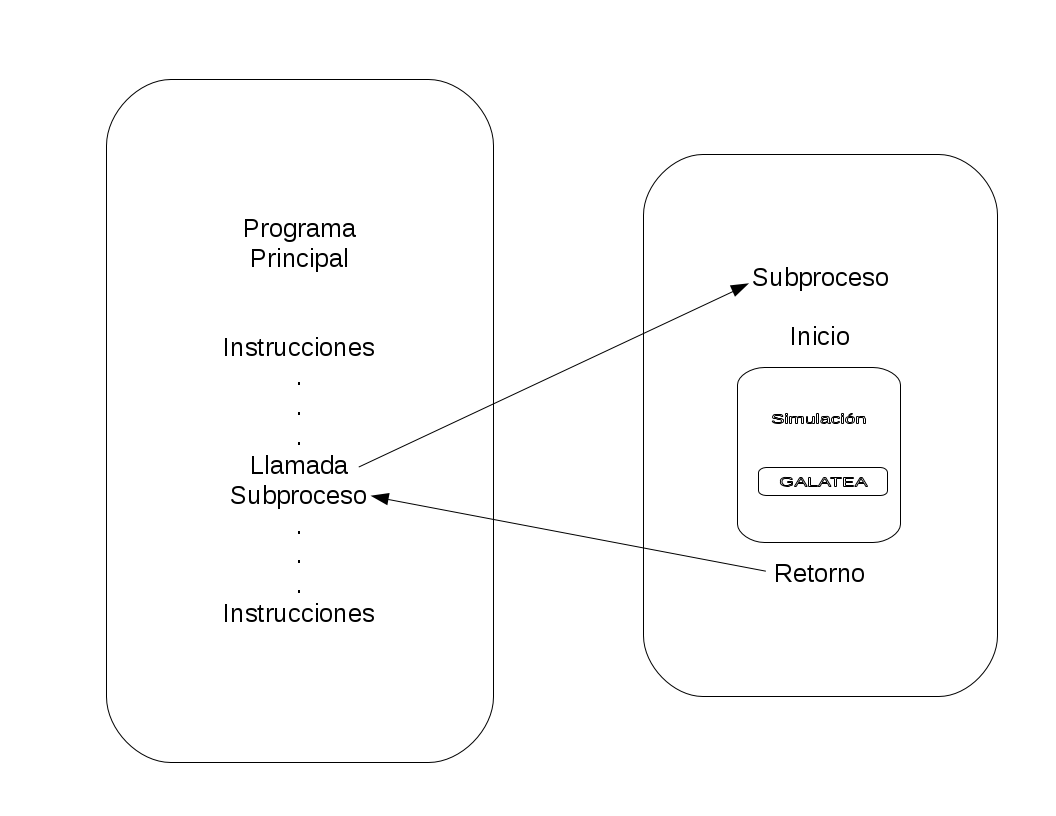
\includegraphics[scale=0.3]{img/estructuraSubproceso.png}
    		\caption{Ejecución de un Subproceso.}
    		\label{subprocesoWork}
    	\end{figure}
    \end{frame}
    \begin{frame}
    	\frametitle{Integración de GALATEA}
    	\framesubtitle{Integración Subprocesos}
    	
    	\begin{itemize}
    		\item Mediante una llamada a un subproceso dentro de nuestro sistema:
    		\begin{itemize}
    			\item Traducir el lenguaje GALATEA.
    			\item Compilar el modelo.
    			\item Ejecutar la simulación.
    			\item Retornar resultado.
    		\end{itemize}
    	\end{itemize}
    \end{frame}
    \begin{frame}
    	\frametitle{Integración de GALATEA}
    	\framesubtitle{Integración Sockets}
    	
    	\begin{columns}
    		\begin{column}{.4\linewidth}
    			\begin{itemize}
    				\item Programa cliente.
    				\item Programa servidor.
    				\item Protocolo de Comunicación.
    			\end{itemize}
    		\end{column}
    		\begin{column}{.6\linewidth}
    			\begin{figure}[H]
    				\centering
    				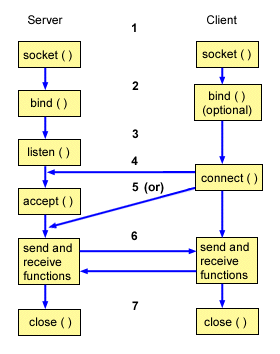
\includegraphics[scale=0.4]{img/socketWork.png}
    				\caption{Típico flujo usando sockets.}
    				\label{socketWork}
    			\end{figure}
    		\end{column}
    	\end{columns}
    \end{frame}
    
    \begin{frame}
    	\frametitle{Integración Sockets}
    	\framesubtitle{Integración Sockets}
    	
    	\begin{figure}[H]
    		\centering
    		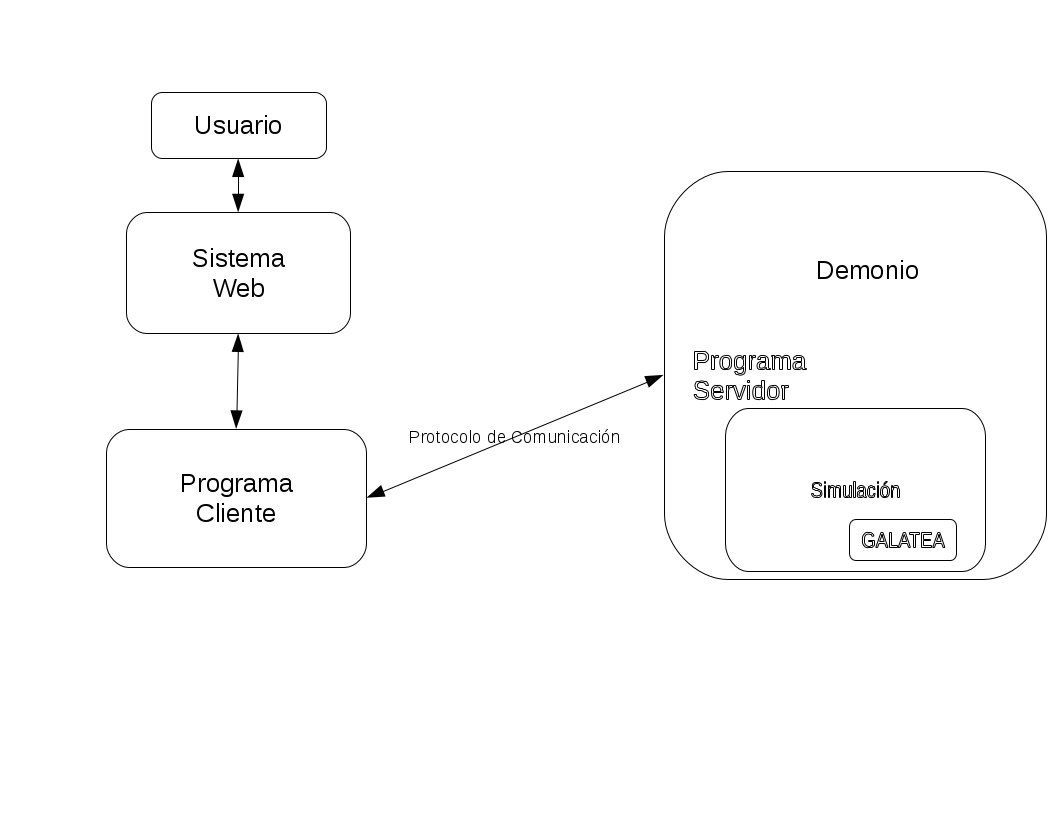
\includegraphics[scale=0.3]{img/estructuraSockets.png}
    		\caption{Estructura Integración mediante Sockets.}
    		\label{estructuraSokets}
    	\end{figure}
    \end{frame}
    \begin{frame}
    	\frametitle{Integración Sockets}
    	\framesubtitle{Programa Servidor}
    	
    	\begin{columns}
    		\begin{column}{.3\linewidth}
    			\begin{itemize}
    				\item Programa servidor.
    				\begin{itemize}
    					\item Manejador de Eventos.
    					\item Hilo de Simulación.
    					\item Cuerpo Principal.
    				\end{itemize}
    			\end{itemize}
    		\end{column}
    		\begin{column}{.7\linewidth}
    			\begin{figure}[H]
    				\centering
    				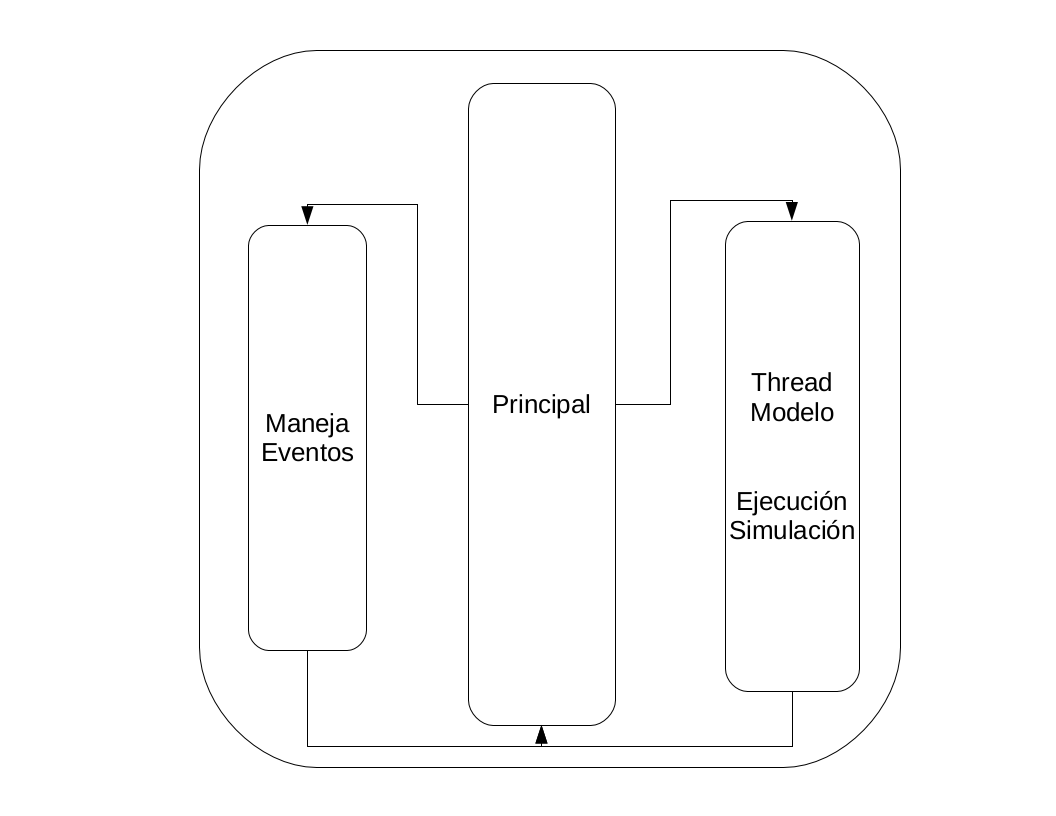
\includegraphics[scale=0.25]{img/estructuraProgramaServidor.png}
    				\caption{Estructura del Programa Servidor.}
    				\label{estructuraProgramaServidor}
    			\end{figure}
    		\end{column}
    	\end{columns}
    \end{frame}
    \begin{frame}
    	\frametitle{Integración Sockets}
    	\framesubtitle{Protocolo de Comunicación}
    	
    	\begin{itemize}
    		\item Protocolo de Comunicación.
    		\begin{itemize}
    			\item Start.
    			\item Sleep.
    			\item Stop.
    			\item Yield.
    			\item Pause.
    			\item Set var.
    			\item Get var.
    		\end{itemize}
    	\end{itemize}
    \end{frame}
    \begin{frame}
    	\frametitle{Integración de GALATEA}
    	\framesubtitle{Resumen}
    	
    	\begin{itemize}
    		\item Subprocesos.
    		\begin{itemize}
    			\item Llamadas.
    			\item Control de eventos.
    		\end{itemize}
    		\item Sockets.
    		\begin{itemize}
    			\item Programa cliente.
    			\item Programa servidor.
    			\item Protocolo de Comunicación.
    		\end{itemize}
    	\end{itemize}
    	
    \end{frame}
    %%------------------------Fin------------------------%%

    %%--------------------Diapositiva--------------------%%
    \section{Pruebas}
    \begin{frame}
        \frametitle{Pruebas}
        %%\framesubtitle{Subtítulo del frame (no obligatorio)}
        
        \begin{itemize}
        	\item Sistema Web.
        	\item Manejo de Archivos.
        	\item Integración de GALATEA.
        	\begin{itemize}
        		\item Subprocesos.
        		\item Sockets.
        	\end{itemize}
        \end{itemize}
    \end{frame}
    \begin{frame}
    	\frametitle{Pruebas}
    	\framesubtitle{Sistema Web}
    	
    	\begin{itemize}
    		\item Sistema Web (JMeter).
    		\begin{itemize}
    			\item Páginas web y archivos estáticos: 640 peticiones por minuto.
    			\item Páginas dinámicas con Django: 768 peticiones por minuto.
    			\item Páginas estáticas dinámicas con Django: 128 peticiones por minuto
    		\end{itemize}
    	\end{itemize}
    \end{frame}
    \begin{frame}
    	\frametitle{Pruebas}
    	\framesubtitle{Integración GALATEA}
    	
    	\begin{itemize}
    		\item Integración GALATEA (Subprocesos).
    		\begin{itemize}
    			\item Variación de argumentos de simulación.
    			\item tSim: el tiempo de simulación variando desde su valor por omisión hasta diez veces ese valor (100).
    			\item InArrTime: tiempo entre llegadas variando desde su valor por omisión hasta el doble de ese valor(8.0).
    			\item MeSerTime: tiempo de servicio variando desde su valor por omisión hasta el doble de ese valor(7.0).
    		\end{itemize}
    	\end{itemize}
    \end{frame}
    \begin{frame}
    	\frametitle{Pruebas}
    	\framesubtitle{Integración GALATEA}
    	
    	\begin{itemize}
    		\item Integración GALATEA (Sockets).
    		\begin{itemize}
    			\item Cliente Python.
    			\item Cliente Java.
    			\item Cliente C.
    			\item Cliente Web.
    		\end{itemize}
    	\end{itemize}
    \end{frame}
    %%------------------------Fin------------------------%%
    
    %%--------------------Diapositiva--------------------%%
    \section{Uso de Sistema}
    \begin{frame}
    	\frametitle{Uso del Sistema}
    	%%\framesubtitle{Subtítulo del frame (no obligatorio)}
    	
    	\begin{itemize}
    		\item Video Inicial.
    		\item Video Registro Usuarios.
    		\item Video Manejo de Archivos.
    		\item Video Compartir archivos y Amigos.
    		\item Video Propuesta de Integración
    	\end{itemize}
    	
    \end{frame}
    %%------------------------Fin------------------------%%
    
    
    %%--------------------Diapositiva--------------------%%
    \section{Conclusiones y Recomendaciones}
    \begin{frame}
    	\frametitle{Conclusiones}
    	%%\framesubtitle{Subtítulo del frame (no obligatorio)}
    	
    	\begin{itemize}
    		\item Sistema web de simulación cuya base principal es GALATEA.
    		\item Sistema de administración de archivos y carpetas.
    		\item Interacción de usuarios dentro del sistema.
    		\item Tecnologías y herramientas de software como: Django, GALATEA, Trello, Git, Github, Apache, Nginx, MySQL, PostgreSQL.
    		\item Se desarrollaron y presentaron dos enfoques de integración (Subprocesos y Sockets).
    		\item Se espera que con este trabajo el universo de usuarios y usuarias de simulación crezca.
    	\end{itemize}
    	
    \end{frame}
    \begin{frame}
    	\frametitle{Recomendaciones}
    	%%\framesubtitle{Subtítulo del frame (no obligatorio)}
    	
    	\begin{itemize}
    		\item Integrar un sistema de educación a distancia para simulación.
    		\item Desarrollar nuevas mejoras en la api de integración de GALATEA para no solo garantizar una comunicación con el sistema web, sino con otros sistemas.
    		\item Red social de simulación.
    		\item Definir e implementar un sistema de control de eventos en tiempo real para GALATEA.
    	\end{itemize}
    	
    \end{frame}
    \begin{frame}
    	\frametitle{Finalización}
    	%%\framesubtitle{Subtítulo del frame (no obligatorio)}
    	
    	{\Huge Gracias}...
    	
    \end{frame}
    %%------------------------Fin------------------------%%

\end{document}